\chapter{Power Series}
\chapter*{Lecture 35}

\begin{recall}{}{}
\begin{itemize}
\item Discussed application of Laplace Transform 
\end{itemize}
\end{recall}





\section{Review of Taylor series expansion}

Suppose a function $f(x)$ has a power series representation about $x=a$:
\begin{equation}
f(x)=\sum_{n=0}^{\infty}c_{n}(x-x_0)^{n}=c_{0}+c_{1}(x-x_0)+c_{2}(x-x_0)^{2}+c_{2}(x-x_0)^{2}+\hdots
\label{Taylor}
\end{equation}
If we evaluate the function at $x=x_0$, we have: $f(x_0)=c_{0}$.
By evaluating the first derivative, we obtain:
\begin{equation*}
f'(x)=c_{1}+2c_{2}(x-x_0)+3c_{2}(x-x_0)^{2}+\hdots
\end{equation*}
and  at $x=x_0$, we have: $f'(x_0)=c_{1}$.
By evaluating the second derivative:
\begin{equation*}
f''(x)=2c_{2}+3\cdot 2 c_{3}(x-x_0)+4\cdot 3 c_{4}(x-x_0)^{2}+\hdots
\end{equation*}
We see that: $\boxed{c_{n}=\frac{f^{(n)}(x_0)}{n!}}$



We can rewrite our power expansion \eqref{Taylor}  as a Taylor series about $x=x_0$ as:
\begin{equation*}
\boxed{P_n(x)=f(x)=\sum_{n=0}^{\infty}\frac{f^{(n)}(x_0)}{n!}(x-x_0)^{n}}
\end{equation*}
or:
\begin{equation*}
f(x)=f(x_0)+f'(x_0)(x-x_0)+\frac{f''(x_0)}{2!}(x-x_0)^{2}+\frac{f'''(x_0)}{3!}(x-x_0)^{3}+\hdots
\end{equation*}

\begin{center}
\line(1,0){250}
\end{center}
\subsection*{Let's foreshadow a bit of MTE204}
Now let's look at a discrete form of the above as $x_0=x_{i}$ (point $i$ on the discretized grid) and $x=x_{i}+\Delta x$ where $\Delta x$ is small
\begin{figure}
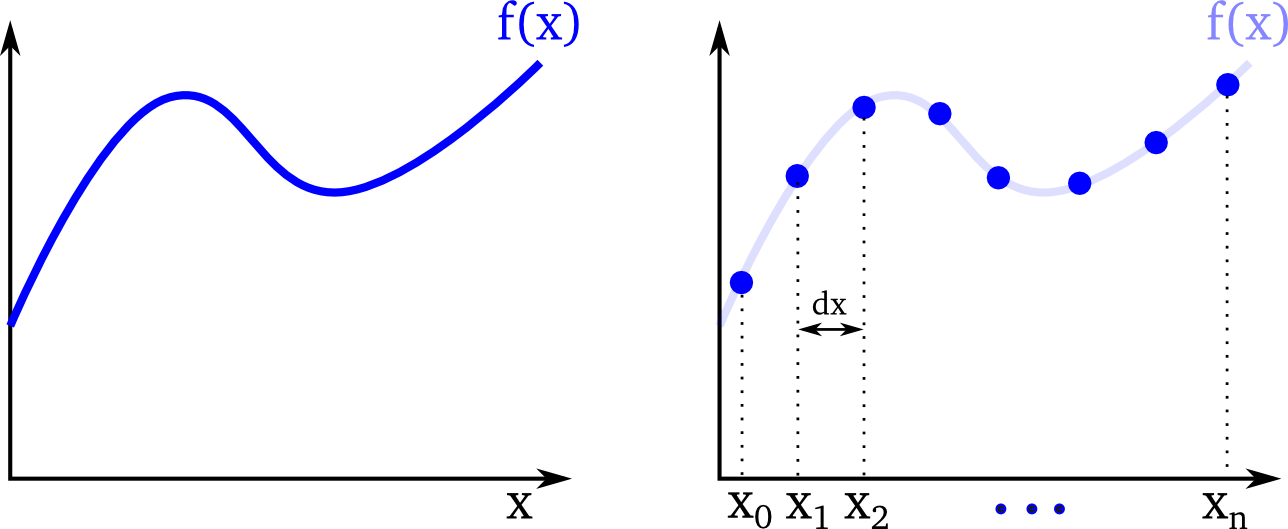
\includegraphics[width=\textwidth]{figs/discretization.png}\par
\end{figure}
\begin{center}
Notation: 
\begin{equation*}
\boxed{f_i=y_i=y(x_i)}
\end{equation*}
\end{center}

\begin{equation*}
f(x_{i}+\Delta x)=f(x_{i})+f'(x_{i})\Delta x+\frac{f''(x_{i})}{2!}\Delta x^{2}+\frac{f'''(x_{i})}{3!}\Delta x^{3}+\hdots
\end{equation*}

Forward looking:
\begin{equation*}
f_{i+1}=f_{i}+\Delta x f'_{i}+\Delta x^{2} \frac{f''_{i}}{2!}+\Delta x^{3} \frac{f'''_{i}}{3!}+\hdots
\end{equation*}
Backward looking:
\begin{equation*}
f_{i-1}=f_{i}-\Delta x f'_{i}+\Delta x^{2} \frac{f''_{i}}{2!}-\Delta x^{3} \frac{f'''_{i}}{3!}+\hdots
\end{equation*}

Note the alternating sign! As complementary work, derive the Taylor series expansion for $x=x_{i}-\Delta x$ to obtain the backward series.



We rearrange the Taylor series to isolate the derivative:
\begin{equation*}
f'_{i}=\frac{f_{i+1}-f_{i}}{\Delta x} - \frac{\Delta x}{2} f''(x_{i})+\hdots
\end{equation*}
If we assume that $\Delta x$ is small, therefore $\Delta x^{2}$ should be much smaller. To a \textbf{first-order}, we can neglect the higher-order terms to obtain a \textbf{forward difference}:
\begin{equation*}
f'_{i}=\frac{f_{i+1}-f(i)}{\Delta x} +O(\Delta x)
\end{equation*}
A first-order backward difference can also be obtained:
\begin{equation*}
f'_{i}=\frac{f_{i}-f_{i-1}}{\Delta x} +O(\Delta x)
\end{equation*}
\begin{center}
\line(1,0){250}
\end{center}


\begin{exmp}{}
Find the Taylor series expansion of:
\begin{equation*}
f(x)=e^x \qquad \qquad \text{about }x_0=0
\end{equation*}
\textbf{Solution:} for $x_0=0$ find $f^{(n)}(x_0)=f^{(n)}(0)$. Since $f^{(n)}(0)=e^0=1$, our power series becomes:
\begin{align*}
P_n(x)=\sum^\infty_{n=0}\frac{f^{(n)}(x_0)}{n!}(x-x_0)^n=\sum^\infty_{n=0}\frac{1}{n!}x^n
\end{align*}
\end{exmp}


\begin{exmp}{}
Find the Taylor series expansion of:
\begin{equation}
f(x)=e^x \qquad \qquad \text{about }x_0=-4
\end{equation}
\textbf{Solution:} for $x_0=-4$ find $f^{(n)}(x_0)=f^{(n)}(-4)=e^{-4}$:

\begin{align*}
P_n(x)=\sum^\infty_{n=0}\frac{f^{(n)}(-4)}{n!}(x+4)^n=E^{-4}\sum^\infty_{n=0}\frac{1}{n!}(x+4)^n
\end{align*}
\end{exmp}




\begin{exmp}{}
Find the 4th-degree Taylor series expansion of $\cos x$ at $x_0=2$.

\textbf{Solution:}The power series will take the following form:
\begin{align*}
P_n(x)=f(x_0)+ f'(x_0)(x-x_0)+ \frac{1}{2!}f''(x_0)(x-x_0)^2+ \frac{1}{3!}f'''(x_0)(x-x_0)^3+ \frac{1}{4!}f^{(4)}(x_0)(x-x_0)^4
\end{align*}
We have:

\begin{align*}
&x_0=2\\
&f(x_0)=\cos(2)\\
&f'(x_0)=-\sin(2)\\
&f''(x_0)=-\cos(2)\\
&f'''(x_0)=\sin(2)\\
&f^{(4)}(x_0)=\cos(2)\\
\end{align*}

Therefore, our solution is:
\begin{align*}
P_n(x)=\cos (2)+ [-\sin(2)](x-2)+ \frac{1}{2!}[-\cos(2)](x-2)^2\\+ \frac{1}{3!}[\sin(2)](x-2)^3+ \frac{1}{4!}[\cos(2)](x-2)^4
\end{align*}
\end{exmp}

%\end{exmp}